% Main document. Here, we import all the necessary packages and create the basic structure of the document. All the text is distributed over other documents to prevent unreadable code.

\documentclass[xcolor=svgnames]{beamer} %add `handout' to options to ignore <+-> and pauses

    \usepackage[utf8]{inputenc}
    \usepackage[english]{babel} 
    
    \usepackage{listings}
    \usepackage{tabularx}
    \usepackage{graphicx}
    \usepackage{wrapfig}
    \usepackage{units}
    \usepackage{comment}
    
    % Nice unnumbered footnotes with \blfootnote
\newcommand\blfootnote[1]{%
  \begingroup
  \renewcommand\thefootnote{}\footnote{#1}%
  \addtocounter{footnote}{-1}%
  \endgroup
}
    
    \usepackage{fixltx2e}
	
	\usetheme{Sybila}
	\title{Sybila Theme Example Document}
	\author{Oliver Conzen (miladiir)}
	\institute{Github Example}
	\date{\today}
 
\begin{document}

\frame[plain]{\titlepage}

\section{Example Section}
\subsection{Basics}
\begin{frame}{\insertsection} % instead of the section, you can title frames whatever you want. for the first frame of a section, this here is really new though
	\framesubtitle{\insertsubsection} % you have to set the subtitle `manually' unfortunately
	\begin{itemize}[<+->] % reveals one point at a time
		\item This is a basic itemization
		\item Only one point at a time
		\item Even \pause pauses \pause in midsentence and \pause points. % pause for manual pause
    \end{itemize}
    \pause \textbf{Everything looks neat and simple.}
\end{frame}

\subsection{Some more}
\begin{frame}{\insertsection}
	\framesubtitle{\insertsubsection}
	\begin{figure}[h]
		\centering
		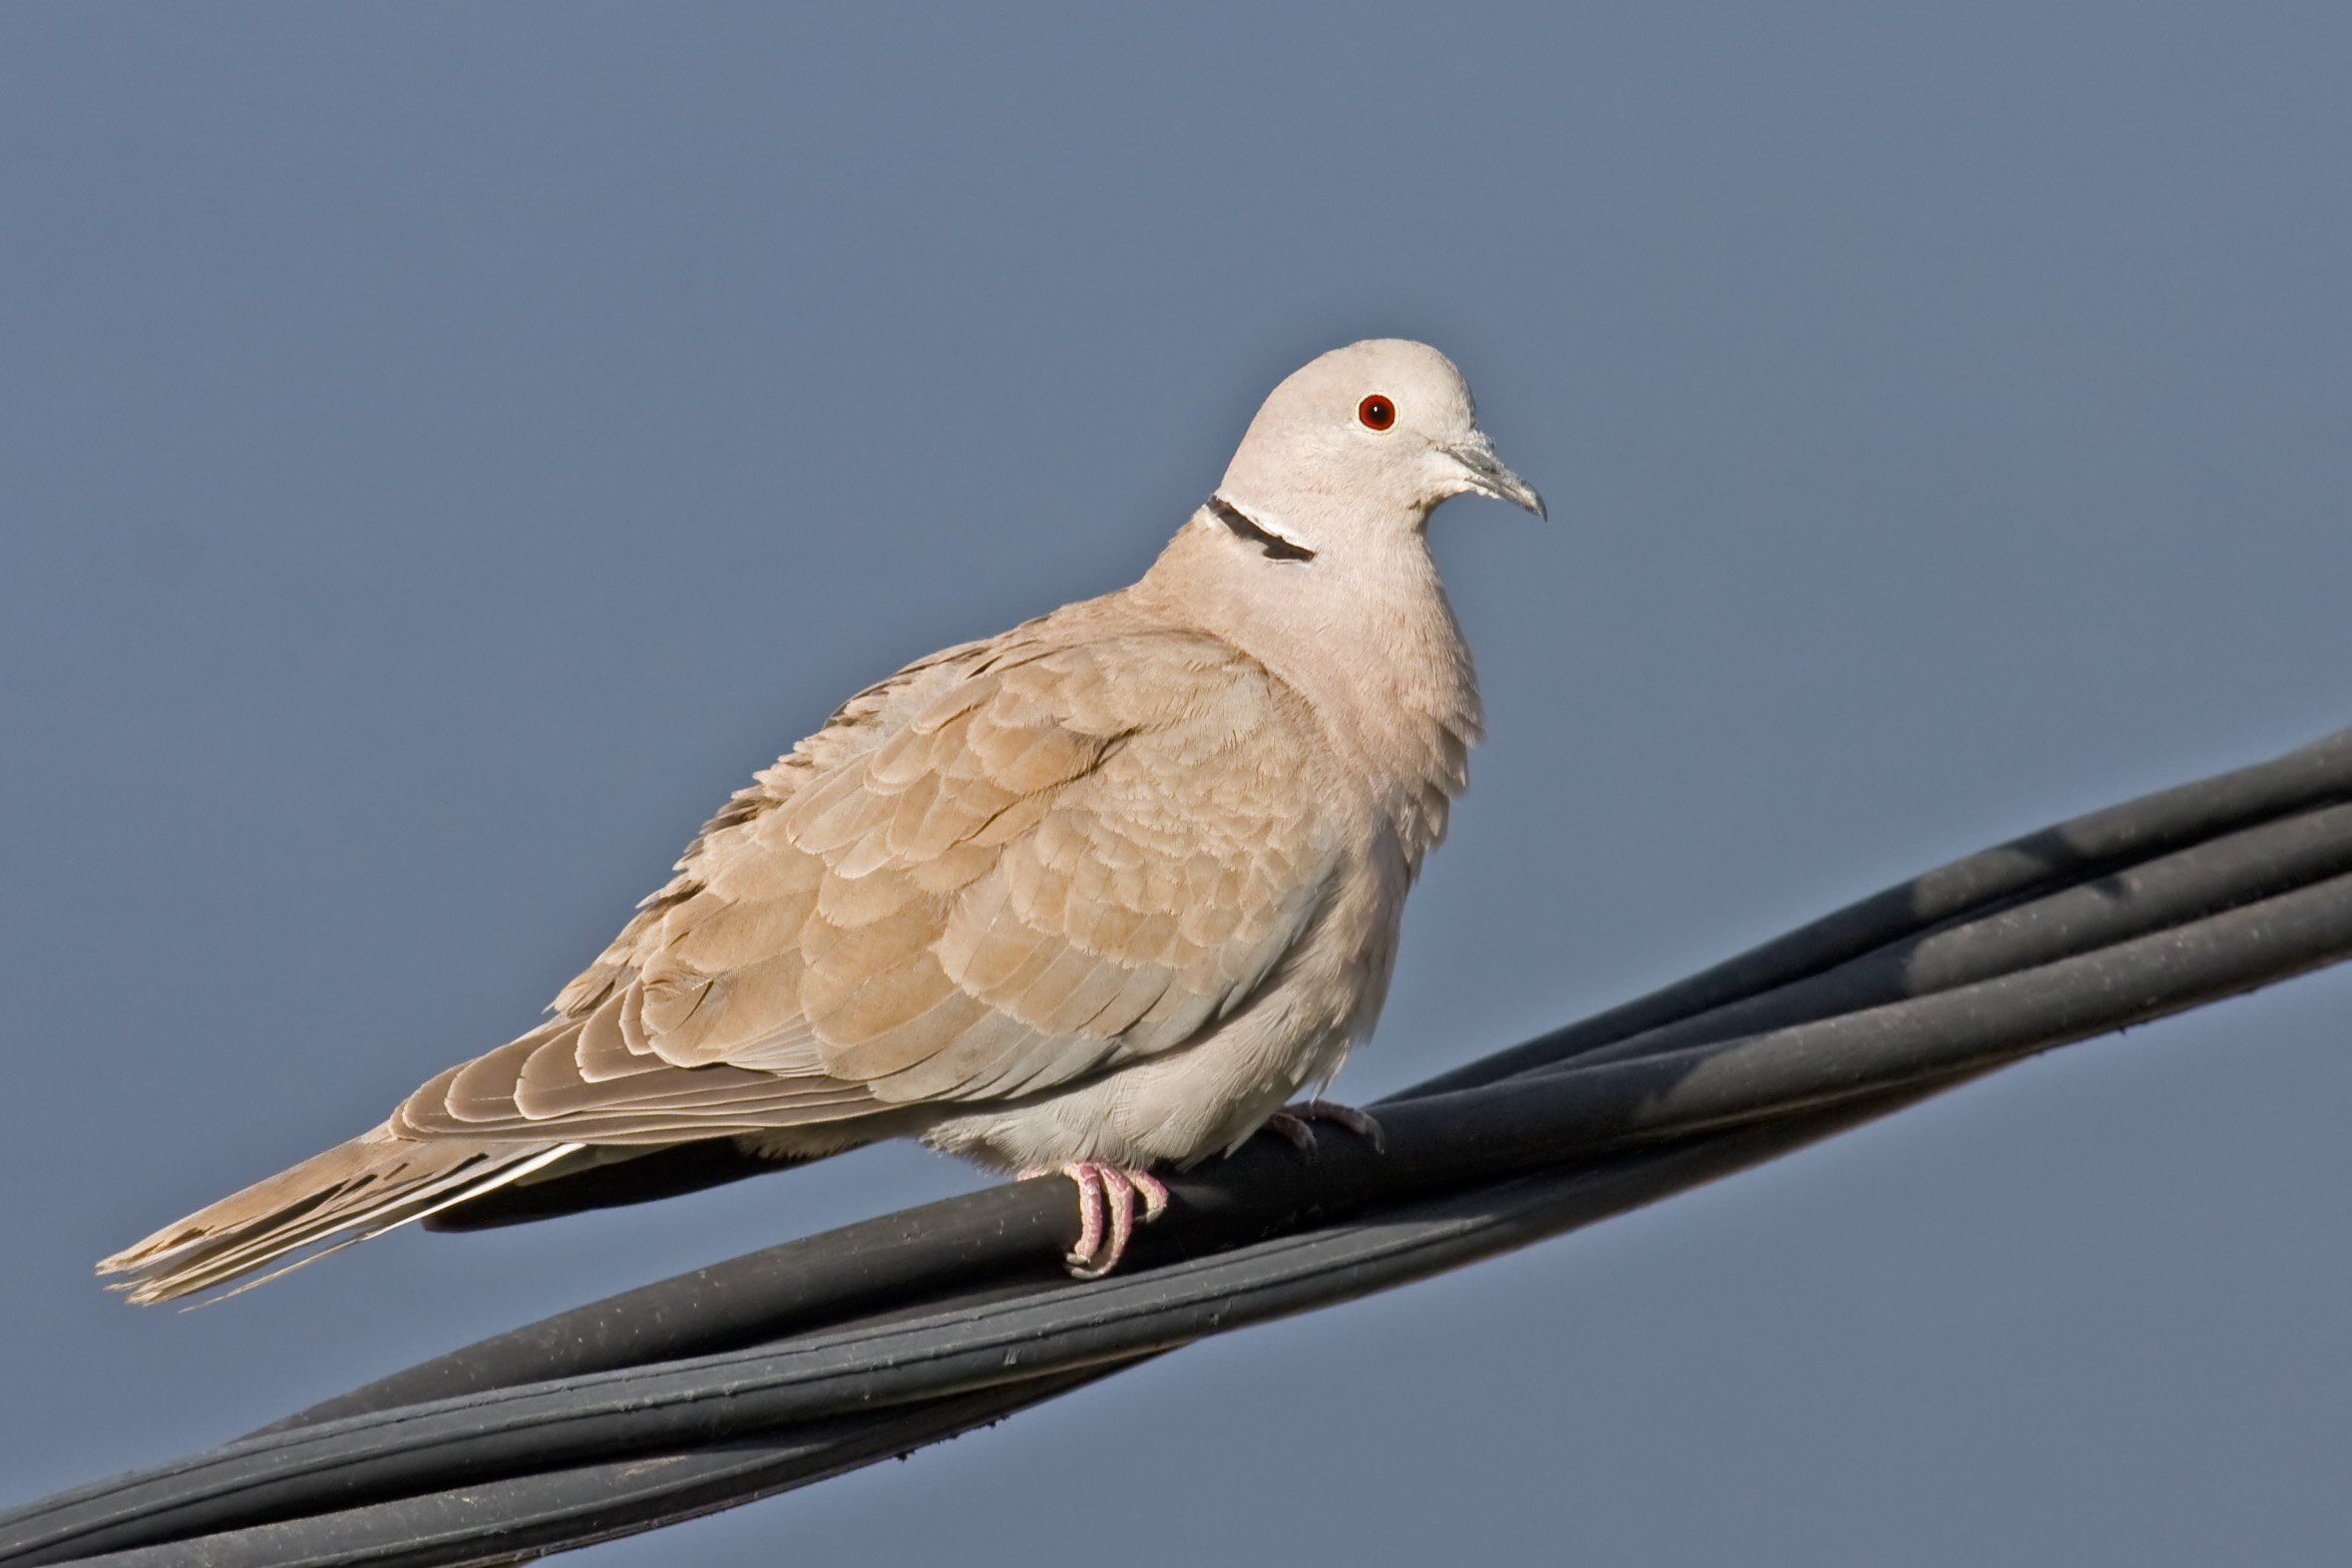
\includegraphics[width=0.7\textwidth,]{Collared_Dove.jpg}
	\end{figure}
	\blfootnote{You can also move the caption of a figure to the frame title or subtitle for a cleaner look.}
\end{frame}

\section{Conclusion}
\begin{frame}{Want some more?}

You can always contact me for questions or use Github Issues.

\vspace{\fill}

\LARGE {\insertauthor} \\
\texttt{oliverconzen@me.com}

\end{frame}
	
\end{document}

% I hope you like it!